\chapter{Grundlagen}\label{ch:grundlagen}
Um den Unterschied zwischen modernen cloud native Entwicklungsprozessen und dem Mainframe Entwicklungsprozess darstellen zu können, werden zunächst Begriffe aus dem cloud-native-Umfeld erläutert.
Dabei wird auch auf den dadurch ermöglichten Entwicklungsprozess, dessen Vorteile und Begrifflichkeiten eingegangen.
Anschließend werden für die Beantwortung der Forschungsfragen relevanten Begriffe des Mainframe-Umfelds beleuchtet.

\section{cloud-native bei der DATEV e.G.}
Eine cloud-native Anwendung ist eine speziell für das Cloud-Computing\footnote{Glossar \ref{Glossar}} konzipierte und entwickelte Anwendung.
Eine solche Anwendung setzt sich meinst aus viele kleine Teile, sogenannte \glqq Microservices\grqq, zusammen.
Diese einzelnen entkoppelten Services sind in Container paketiert.
Diese Container und somit die Anwendung können auf verschiedenen Cloud-Umgebungen, auch von unterschiedlichen Anbietern,  ausgeführt werden.
Dadurch ist eine schnelle Reaktion auf Markt- und Kundenanforderungen möglich.
Außerdem besteht keine Herstellerabhängigkeit.\cite{cloudnative.23.2.2020}\\
Eine moderne cloud-native Anwendung innerhalb der DATEV e.G. machen folgende Dinge aus:
\begin{itemize}
\item \glqq Cloud Foundry\grqq
\item CI/CD-Pipeline
\end{itemize}

\section{\glqq Cloud Foundry\grqq}
Bei Cloud Foundry handelt es sich um eine quelloffene Platform-as-a-Service, kurz PaaS.
Platform-as-a-Service, beschreibt neben Insfrastructure-as-a-Service, kurz IaaS und Software-as-a-Service, kurz SaaS, einen Grad an Auslagerung von IT-Systemen in die Cloud.
Im Vergleich zu SaaS, bei der ganze Anwendungen in einer Cloud zur Verfügung stehen, stellt eine PaaS-Lösung eine Plattform, die sich neben der Infrastruktur auch um das Betriebssystem, die Middleware und die Laufzeitumgebung kümmert, bereit.
Für die Verwaltung von Ressourcen bietet Cloud Foundry eine Weboberfläche, den sogenannten \glqq Marketplace\grqq, an.
In diesem können mit wenigen Mausklicks Schnittstellen zu Datenbankmanagementsysteme oder Monitorlösungen zur Anwendung hinzugefügt werden.
Diese Schnittstellen, auch \glqq Self-Service\grqq{} oder \glqq Service-Broker\grqq{} genannt, können mittels einer von Cloud Foundry zur Verfügung gestellten API selbst entwickelt werden.
Ein Vorteil ist, dass sich Cloud Foundry um das Staging der Anwendungen kümmert.
Um eine Anwendung in eine solche Stage bereitzustellen, bietet Cloud Foundry ein Kommandozeileninterface an.
Neben der Bereitstellung können mit diesem Interface beispielsweise Anwendungen auch horizontal skaliert werden.
Um die Breitstellung über mehrere Stages hinweg zu automatisieren komm bei der DATEV e.G. eine auf Jenkins basierende CI/CD-Pipeline zum Einsatz.
\cite{foundry.23.2.2020}

\section{\glqq CI/CD-Pipeline\grqq}

\section{Mainframe / Großrechner}\label{sec:mainframe}
Im modernen Sprachgebrauch kann ein Großrechner oder auch Mainframe als größte zur Verfügung stehende Serverart betrachtet werden.
Er wird von Unternehmen verwendet, um  kommerzielle Datenbanken, Transaktionsserver und Anwendungen, die einen hohen Grad an Sicherheit und Verfügbarkeit benötigen, zu hosten.
Im Gegensatz zu verteilten Serversystemen, bei denen die Funktionalitäten auf einzelne Server, wie zum Beispiel einen E-Mail-Server, einen Datenbank-Server, einen Web-Server usw. aufgeteilt sind, handelt es sich bei einem Mainframe um ein zentralisiertes System.
Die einzelnen Funktionalitäten werden von sogenannte \glqq Subsysteme\grqq, auch \glqq Middleware\grqq{} genannt, zur Verfügung gestellt.
Darunter zählen unter anderem Datenbanksysteme und Anwendungsserver.
\cite{Ebbers.2011}

\section{Mainframe Anwendungen bei DATEV e.G.}\label{sec:zosanw}
Das Betriebssystem des IBM Mainframes ist z/OS.
Darauf aufbauend benötigen klassische z/OS Anwendungen bestimmte Middleware.
Bei der DATEV e.G. handelt es sich unter anderem um folgende Middlewarekomponenten:

\begin{itemize}
\item Laufzeitumgebung: CICS oder Batch
\item Datenhaltung: VSAM oder Db2
\item Message Queuing: IBM MQ
\end{itemize}

Diese Subsysteme stehen in jeder Stage zur Verfügung.
Eine Stage beschreibt eine isolierte Systemumgebung mit eigenen Subsystemen und Ressourcenverwaltung.
Die DATEV e.G. unterscheidet am Mainframe vier Stages:
\begin{samepage}
\begin{itemize}
\item Testplex:\\
Labor für Änderungen am System, beispielsweise einer neuen Betriebssystemsversion
\item Entwicklung:\\
Implementierung neuer Features und Durchführung kleiner Tests
\item Qualitätssicherung:\\
Durchführung von Integrationstests
\item Produktion:\\
Software, die für den Kunden bereitsteht
\end{itemize}
\end{samepage}

\section{Subsysteme / Middleware}
Für die Beantwortung der Forschungsfragen liegt der Fokus auf dem Erstellen (\glqq Provisionieren \grqq) einer anwendungsspezifischen Laufzeitumgebung mit einer Datenhaltung und Message Queuing innerhalb des Testplexes und der Entwicklung.
Als Laufzeitumgebung wird \glqq CICS\grqq, als Datenhaltung \glqq Db2\grqq{} und für das Message Queuing \glqq IBM MQ\grqq{} verwendet.
Wie in Abbildung \ref{fig:archüber} dargestellt ist, existieren mehrere Instanzen pro Subsystem.
Es existiert bei der DATEV e.G. jedoch nur eine geringe Anzahl an Instanzen pro Subsystem.
Diese Instanzen sind langlebig und müssen dahingehend gepflegt und gewartet werden.
Daraus folgt, dass sich, wie in der Problemstellung, Absatz \ref{sec:probstell}, bereits erwähnt, viele Anwendungen die gleichen Test-CICS/Db2/MQ Ressourcen teilen.
Diese einzelnen Subsysteme werden im Folgenden erläutert, hierzu dient Abbildung \ref{fig:archüber} als Überblick.

\begin{figure}[h!]
\centering
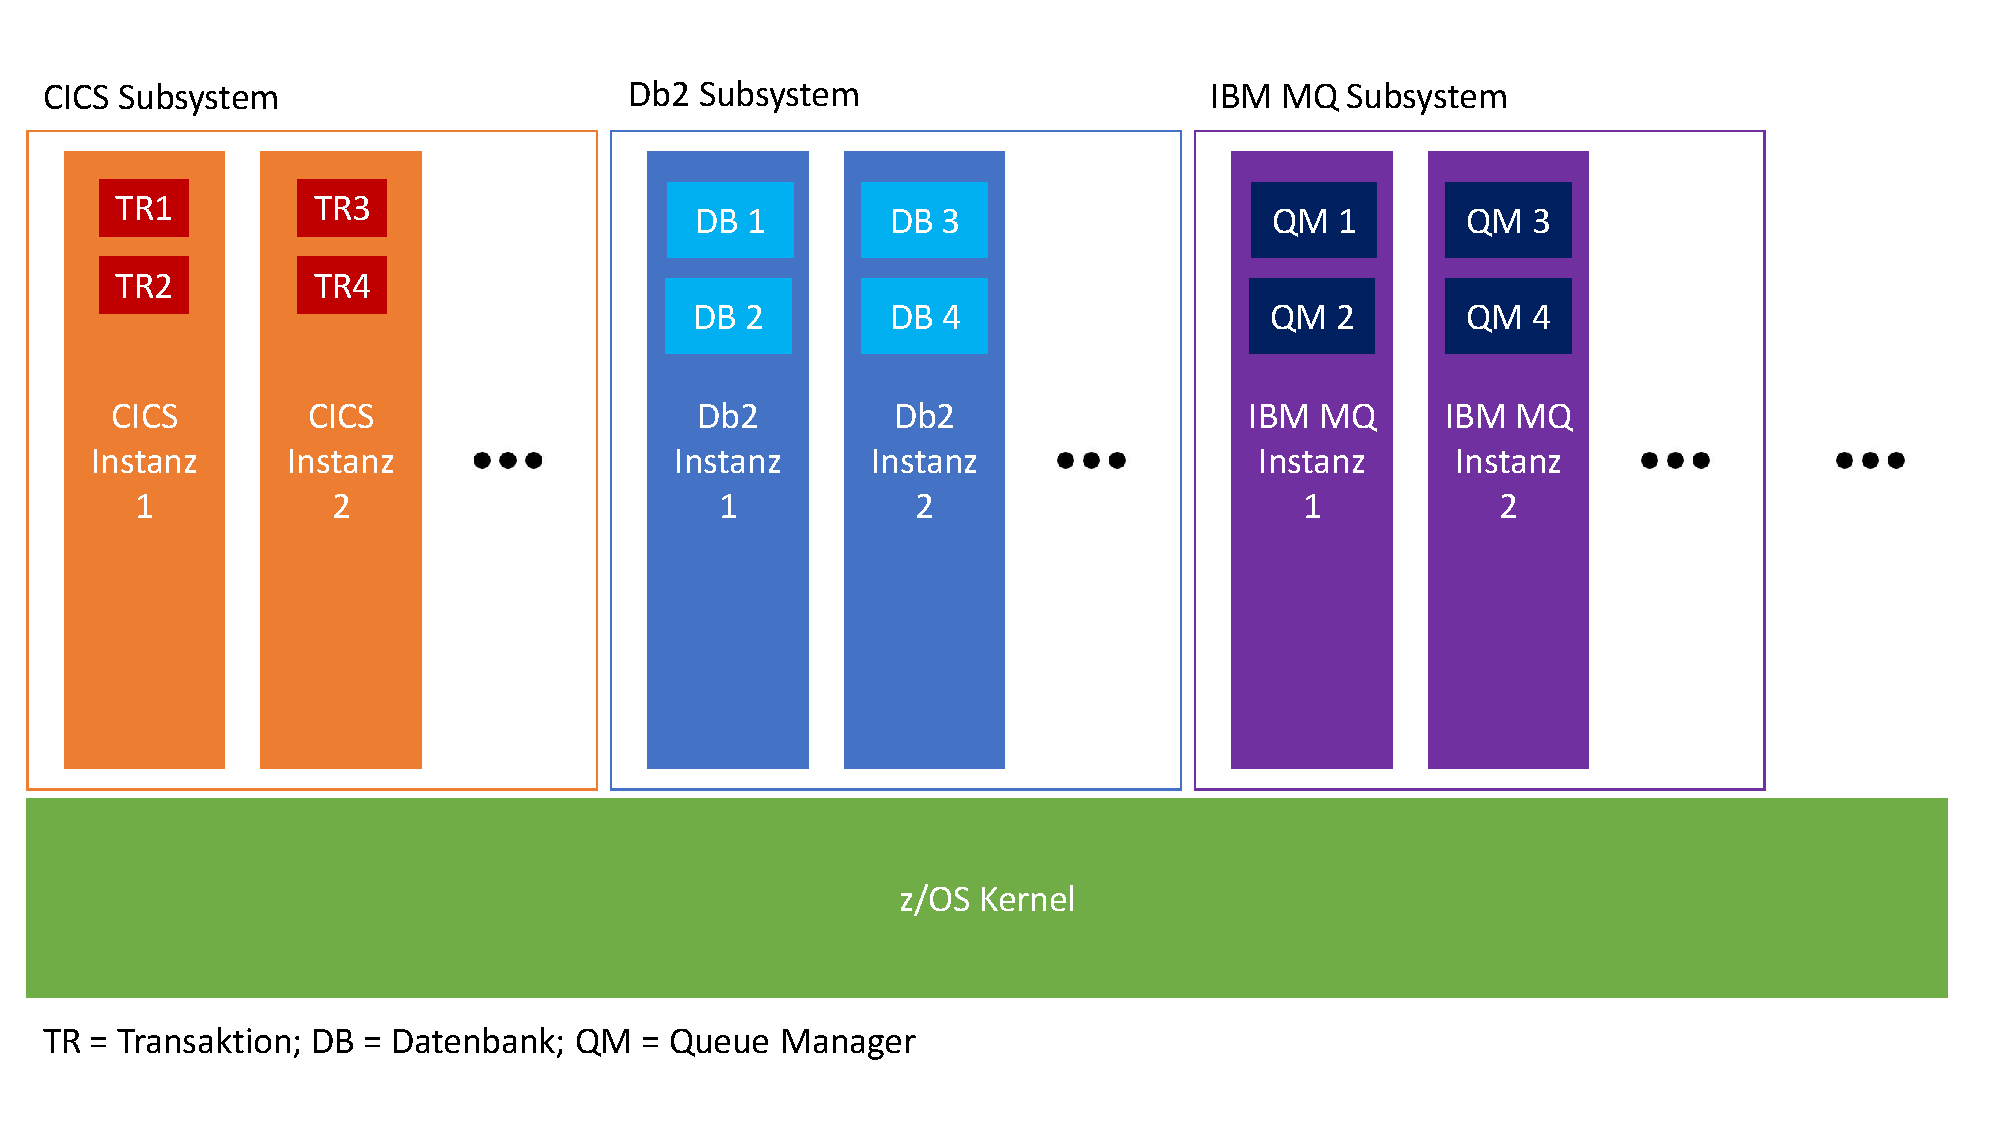
\includegraphics[width=\textwidth]{figures/architektur.pdf}
\caption{Architekturübersicht über die Subsysteme einer Stage bei DATEV eG}
\label{fig:archüber}
\end{figure}

\subsection{Customer Information Control System}\label{cics}
Das Customer Information Control System, kurz CICS, ist ein Applikationsserver für einen IBM-Großrechner mit Betriebssystem z/OS und damit eine IBM Middleware.
Ein Applikationsserver stellt eine Umgebung zur Verfügung, in der Anwendungen gehostet werden können.
Dabei kümmert sich dieser unter anderem um Transaktionalität, Webkommunikation und Sicherheit.
Hierfür stellen Applikationsserver eine API zur Verfügung.
CICS hat einen Vorteil gegenüber anderen Anwendungsservern, es unterstützt verschiedene Programmiersprachen.
CICS ist ein Multi-Language Application Server und unterstützt z.B. COBOL, Assembler, Java und PLI.
So können Programme innerhalb einer Anwendung in der für ihren Use-Case am besten geeigneten Sprache implementiert werden.
\cite{Rayns.2011}

Das CICS Subsystem einer Stage umfasst mehrere CICS Instanzen.

\subsubsection{CICS Instanz} 
Unter einer CICS Instanz ist ein einzelner Bereich, der auf dem z/OS Kernel aufsetzt, zu verstehen.
Dieser Bereich ist mittels einer eindeutigen CICS ApplicationID gekennzeichnet und kann darüber explizit angesprochen werden.
Eine CICS Instanz verwaltet mehrere CICS Transaktionen.

Wenn in dieser Arbeit von dem CICS gesprochen wird, ist die CICS-Instanz damit gemeint.

\subsubsection{CICS Transaktion}\label{subsec:trans}
Ein Businessablauf wird im CICS in einer Transaktion gekapselt.
Eine Transaktion kann mehrere Programme unterschiedlicher Programmiersprachen umfassen und wird über eine eindeutige \glqq TransaktionsID\grqq{} identifiziert..

Über die TransaktionsID wird der Ablauf gestartet.
Dies kann sowohl per Webanfrage oder per Messaging Queue als auch aus einem anderen Programm heraus oder manuell geschehen.
In der Transaktion werden alle Änderungen, die Programme an Ressourcen, wie zum Beispiel einer Datenbank oder Dateien tätigen, protokolliert.
So wird im Falle eines Fehlers die Möglichkeit eines Rollbacks sichergestellt.
 \cite{Rayns.2011}

\subsection{Db2}\label{sssec:db2}
Db2 ist ein relationales Datenbanksystem, welches unter anderem als Subsystem eines z/OS Betriebssystems läuft.
Einer Stage können mehrere Datenbanksysteme, auch Instanzen genannt, zugeordnet werden.
In einer Instanz befinden sich die Datenbanken und Tabellen.

\subsection{IBM MQ}\label{sec:mq}
IBM MQ ist eine Messaging-Lösung der IBM.
Diese ermöglicht den asynchronen Datenaustausch zwischen Anwendungen mittels sogenannter Queues.
Alle IBM MQ Begrifflichkeiten, die in dieser Arbeit verwendet werden, werden im Folgenden erläutert.
\cite{Aranha.2013}

Das IBM MQ Subsystem einer Stage setzt sich aus einem oder mehreren Queue Managern zusammen.
Ein Queue Manager kann daher als IBM MQ Instanz gesehen werden.

\subsubsection{Queue Manager}
Bei einem Queue Manager handelt es sich um die zentrale Ressource eines IBM MQ Systems.
Er verwaltet  alle anderen IBM MQ Ressourcen.
Dazu gehören unter anderem die Speichersteuerung der Daten und die Wiederherstellung dieser im Falle eines Fehlers.
Desweiteren koordiniert er den Zugriff aller Anwendungen auf die Nachrichten in den von ihm verwalteten Queues.
Um hierbei die Konsistenz sicherzustellen, sorgt er für Locking und die notwendige Isolation der Queues.
\cite{Aranha.2013}

\subsubsection{Queues}
In Queues werden die Nachrichten, die von Programmen gesendet und gelesen werden gespeichert.
Es gibt verschiedene Arten von Queues, die im Kontext dieser Arbeit relevanten Queues sind folgende:

\paragraph{Die Local Queue.}~\\
Dabei handelt es sich um die einzige Queue Art, bei der die Nachrichten physikalisch gespeichert werden.
Die anderen Queue Arten nutzen als Basis immer eine Local Queue.

\paragraph{Initiation Queue}~\\
Die sogenannte \glqq Initiation Queue\grqq{} ist eine spezielle Art der Local Queue.
Diese dient dem Queue Manager dazu, unter bestimmten Bedingungen eine Trigger-Nachricht darauf zu schreiben.
Daher kann eine andere Local Queue so definiert sein, dass sobald eine Nachricht auf sie geschrieben wird eine solche Trigger-Nachricht erzeugt wird.
Dies ermöglicht, dass Anwendungen nur starten, wenn wirklich Daten zum Verarbeiten vorhanden sind.
\cite{Aranha.2013}

\subsubsection{Process}
Für das Auslösen von Anwendungen wird nicht nur die Initiation Queue benötigt, sondern auch sogenannte \glqq Processes\grqq.
So muss der Local Queue, die den Start einer Anwendung auslösen soll, bei der Definition nicht nur die Initiation Queue bekannt gemacht werden, sondern auch ein Process.
Ein Process legt den \glqq Type\grqq{} und den Namen der zu startenden Anwendung fest.
Als \glqq Type\grqq{} können beispielhaft CICS oder auch WINDOWSNT für Windows unterstütze Plattformen genannt werden.
Ist der \glqq Type\grqq{} CICS,  muss der Name der Transaktion angegeben werden, für Windows Plattformen der Dateipfad der auszuführenden exe.
\cite{Aranha.2013}

\section{\glqq IBM Cloud Provisioning and Management for z/OS\grqq}
Die Verwaltung von Subsystemen ist mit vielen manuellen Schritten verbunden.\footnote{Analyse des aktuellen Bereitstellungsprozesses, siehe in Absatz \ref{sec:aktbereit}}
Betreut werden die einzelnen Subsysteme über alle Stages hinweg von eigens dafür entstandenen Administratorenteams.
Die \glqq CICS Administration\grqq{} kümmert sich um alles rund um das CICS Subsystem.
Die \glqq Db2 Administration\grqq{} stellt Datenbanken und Tabellen auf Anfrage der Entwickler bereit.
Die \glqq IBM MQ Administration\grqq{} verwaltet die IBM MQ Ressourcen.
Um diese Aufgabe zu bewältigen sind aktuell viele proprietäre und veraltete Tools im Einsatz.

Für die Automation dieser Prozesse bietet die IBM \glqq IBM Cloud Provisioning and Management for z/OS\grqq{} an.
Dabei handelt es ich um ein bei der Installation von \glqq z/OS Management Facility\grqq{}\footnote{Siehe Absatz \ref{sssec:zosmf}}, kurz z/OSMF, mitgeliefertes Tool.
Beide Tools sind innerhalb der DATEV e.G. vorhanden, allerdings werden sie sehr selten genutzt.
Sie sind auch außerhalb der DATEV e.G. kaum verbreitet.
Aus Sicht der IBM besteht Interesse an Erfahrungsberichten zur Nutzung von \glqq IBM Cloud Provisioning and Management for z/OS\grqq.
So wurde im Rahmen der neunzehnten \glqq AMC\grqq{}\footnote{Academic Mainframe Consortium e.V.} Tagung im IBM Client Center Böblingen am 16.01.2020 um ca. 14:30  bei einem ca. 30 minütigen Vortrag ein Arbeitsstand dieser Arbeit vorgestellt.
Die Agenda der Veranstaltung ist im Anhang \ref{app:AMC} zu finden.
Der AMC e.V. ist ein Förderverein für die akademische Ausbildung auf dem Mainframe.\footnote{\cite{Amc.23.2.2020}}
Neben Vertretern der IBM nahmen an der Tagung Vertreter von Hochschulen und verschiedenen Unternehmen teil.
Der Vortrag \glqq kam ja sehr gut an und hat auch später noch zu Gesprächen geführt\grqq\footnote{AMC Vorstand Ernst Lugert, 20.1.2020}.
Daraus lässt sich ableiten, dass sich neben der DATEV e.G. und der IBM auch andere Firmen für die automatisierte Provisionierung von z/OS Middleware mit \glqq IBM Cloud Provisioning and Management for z/OS\grqq{} interessieren.

Bei \glqq IBM Cloud Provisioning and Management for z/OS\grqq{} stehen die sogenannten \glqq Templates\grqq{} im Mittelpunkt.
Mit Hilfe eines Templates können Instanzen erzeugt werden.
Diese Instanz kann eine oder mehrere verschiedene Subsystem-Instanzen enthalten.
Dabei steht eine schnelle Provisionierung als auch Deprovisionierung von Instanzen im Vordergrund.
Mittels Templates läuft diese automatisiert, verlässlich und ohne manuelle Abstimmungen ab.
Dadurch ist die Bereitstellung einer Instanz wiederholbar, so kann die Instanz im Fehlerfall sicher neugestartet werden und muss nicht langlebig gepflegt werden.
\\ Ein solches Template besteht aus drei Dateien:

\paragraph{\glqq Aktiondefinitionfile\grqq} ~\\
Hier werden die Aktionen, die ein Anwender mit einer Instanz eines Templates durchführen kann, festgelegt.
Einer Aktion wird ein sogenannter \glqq Workflow\grqq{} zugewiesen.

Ein Workflow ist über eine XML Datei, die sogenannte \glqq Workflowdefinitionfile\grqq, definiert.
Diese lässt sich grob in zwei Teile untergliedern:
\begin{itemize}
\item Variablendefinition
\item Steps
\end{itemize}
In der Variablendefinition werden, wie der Name schon sagt, alle Variablen, die für diesen Workflow notwendig sind definiert.

Ein Step beschreibt einen Teilablauf eines Workflows.
Ein Workflow kann aus mehreren Steps bestehen.
Die Steps werden in Definitionsreihenfolge ausgeführt.
Allerdings können Bedingungen für die Durchführung eines Steps definiert werden.
So ist es beispielsweise möglich, einen Step nur durchzuführen, wenn eine bestimmte Variable einen bestimmten Wert besitzt.
Innerhalb eines Steps können sowohl interne und externe Scripte als auch JCLs und somit Programme ausgeführt werden.
Darüber hinaus besteht die Möglichkeit REST-Calls auszuführen.
Durch ein XML Schema wird sichergestellt, dass die Workflowdefinitionfile keine syntaktischen Fehler beinhaltet.
Sowohl die Variablendefinition als auch die Steps können in externe XML Dateien ausgelagert werden.
Dadurch können Variablen an einer Stelle im Template definiert und in alle Workflowdefinitionfiles aufgenommen werden.
\cite{Rotthove.2018}

Neben den Workflowdefinitionfiles muss in einer Aktion auch der Pfad der sogenannte \glqq Variableinputfile\grqq{} angegeben sein.

\paragraph{\glqq Variableinputfile\grqq}\label{par:variable} ~\\
In dieser Datei werden den in der Workflowdefinitionfile definierten Variablen Werte zugewiesen.
Somit kann das Template konfiguriert werden.

\paragraph{\glqq Manifest-File\grqq} ~\\
Hier wird dem Template mitgeteilt, an welchem Speicherort sich die oben genannten Dateien befinden.
Da ein Template immer provisioniert werden kann, wird hier auch der Speicherort des Provisionierungsworkflows angegeben.
Zusätzlich kann noch eine Beschreibung des Templates hinzugefügt werden.
\cite{IBM.2019}

Für die Provisionierung eines Templates müssen diesem eine sogenannte \glqq Domain\grqq{} und ein \glqq Tenant\grqq{} zugewiesen werden.
Unter einer \glqq Domain\grqq{} ist ein System zu verstehen, dass Systemressourcen in Ressourcenpools gliedert.
\glqq Tenants\grqq{} sind die dazugehörigen Rechtegruppen, die dem Anwender den Zugriff auf und die Nutzung von zugeordneten Templates ermöglicht.
\cite{Rotthove.2018}

Dies umfasst zwei Lösungen, \glqq z/OS Provisioning Toolkit\grqq\footnote{siehe Absatz \ref{sssec:zospt}} und \glqq z/OS Management Facility\grqq\footnote{siehe Absatz \ref{sssec:zosmf}}.

\subsection{z/OS Provisioning Toolkit}\label{sssec:zospt}
z/OS Provisioning Toolkit, kurz z/OSPT, bietet ein Kommandozeileninterface für die Bereitstellung und das Verwalten von Templates.
In Abbildung \ref{fig:zospt_help} werden die möglichen Kommandozeilenbefehle mittels des Befehls \glqq zospt -h\grqq{} in einem Kommandofenster angezeigt.
\begin{figure}[h]
	\centering
	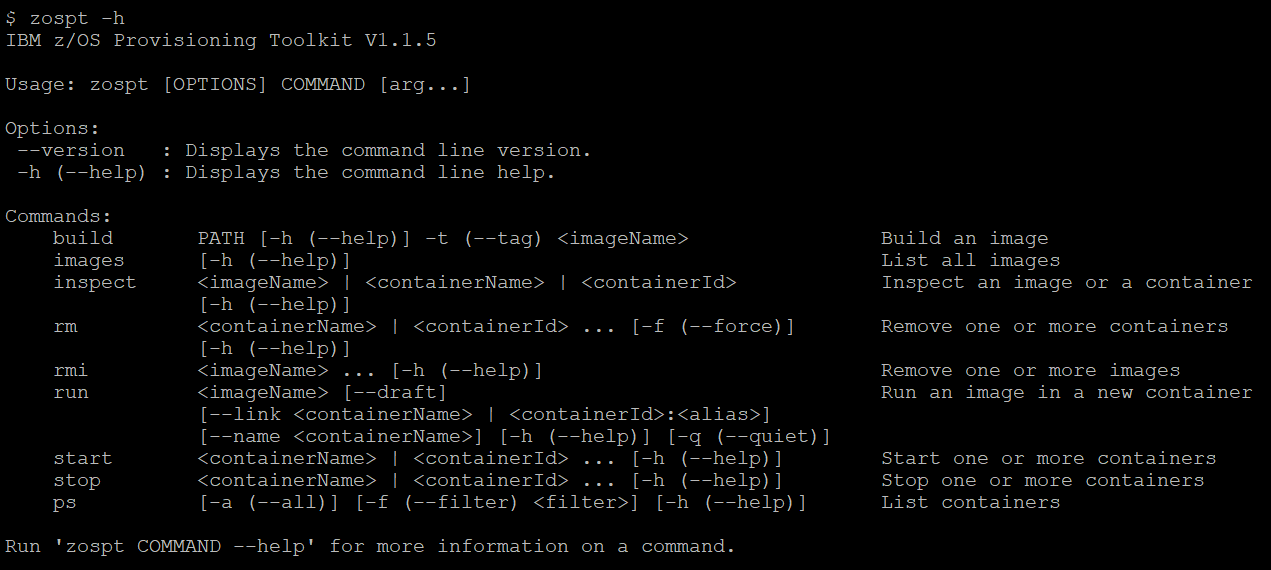
\includegraphics[width=\textwidth]{figures/zospt_help_putty.png}
	\caption{z/OSPT mögliche Kommandozeilenbefehle}
	\label{fig:zospt_help}
\end{figure}
Mit z/OSPT werden zwei weitere Begriffe eingeführt.\\
\paragraph{\glqq Images\grqq}~\\
Dabei handelt es sich grundsätzlich um ein Template, jedoch kann dieses Template über eine weitere Inputdatei verändert werden.
Dadurch kann ein Template mit spezifischen Änderungen provisioniert werden, ohne dass ein neues Template erzeugt werden muss.
Dies erhöht die Flexibilität der Templates weiter.

\paragraph{\glqq Container\grqq}~\\
Dabei handelt es sich um eine Template-Instanz \footnote{Beschreibung in Absatz \ref{sssec:instance}}.
\cite{IBM.2019b}

\subsection{z/OS Management Facility}\label{sssec:zosmf}
Der Funktionsumfang von z/OS Management Facility, kurz z/OSMF, umfasst Systemmanagementfunktionen in einer browserbasierenden Benutzeroberfläche, dargestellt in Abbildung \ref{fig:zosmf_welcome}.
Zu diesen Funktionen zählt die Verwaltung von Workflows und Templates.

\begin{figure}[h]
\centering
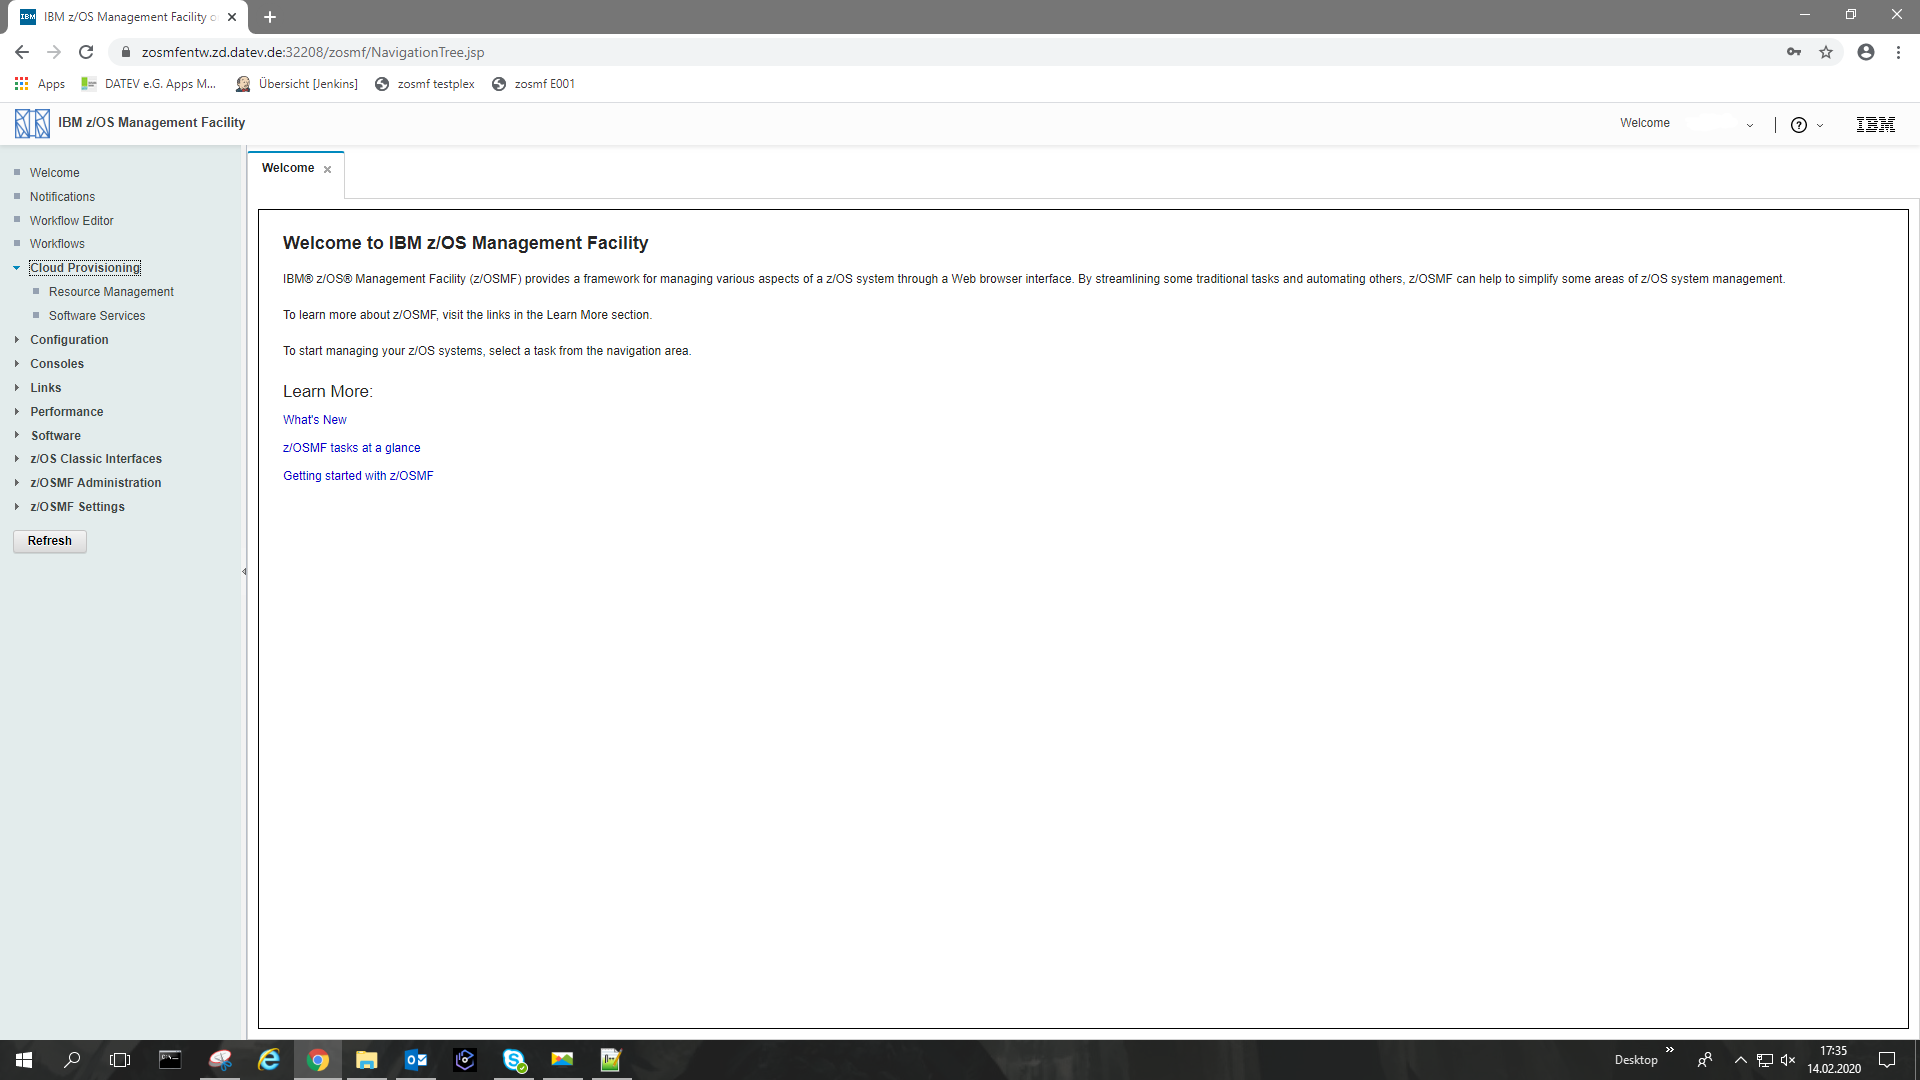
\includegraphics[width=\textwidth]{figures/zosmf.png}
\caption{z/OSMF Willkomens Ansicht}
\label{fig:zosmf_welcome}
\end{figure}

Die linke Seite der Abbildung \ref{fig:zosmf_welcome} zeigt den Umfang der z/OSMF  Funktionen.
Für diese Arbeit besitzt nur der Menüpunkt \glqq Cloud Provisioning\grqq{} Relevanz.
Unter diesem Punkt sind die Funktionalitäten für die automatisierte Bereitstellung von Templates zu finden.
\cite{Rotthove.2018}

Zuerst ist das \glqq Resource Management\grqq{} zu nennen.
Hier werden die \glqq Domains\grqq{} und \glqq Tenants\grqq{} verwaltet.
Zur Verwaltung der Templates und Template-Instanzen kommen die \glqq Software Services\grqq{} zum Einsatz.
Dort können neue Templates über die Manifest-File hinzugefügt werden.
Dann muss, wie oben beschrieben, eine \glqq Domain\grqq{} und ein \glqq Tenant\grqq{} zugwiesen werden.
Anschließend kann das Template, falls es keine Fehler beinhaltet, veröffentlicht werden.
Es ist zu empfehlen vorher einen \glqq Test Run\grqq{} durchzuführen.
Dabei wird eine Instance testweise provisioniert.
Diese Template-Instanz verhält sich genauso wie eine Instanz, die aus einem veröffentlichten Template erzeugt wurde.
Somit können damit das Template und die in der Aktiondefintionfile definierten Aktionen getestet werden.
\cite{Rotthove.2018}
